%! TEX program = xelatex
\documentclass[UTF8]{ctexbeamer}
\usetheme{CambridgeUS}
\usecolortheme{dolphin}
% \definecolor{myorange}{RGB}{255,127,0}
% \setbeamercolor{structure}{fg=myorange}

\usepackage{xeCJK}
\setCJKmainfont{Noto Serif CJK SC}
\setCJKsansfont{Noto Sans CJK SC}

\usepackage{pgfplots}
\pgfplotsset{compat=newest}

\title{中文 Beamer 测试}
\author{你的名字}

\begin{document}

\begin{frame}
  \titlepage
\end{frame}

\begin{frame}{目录}
  \tableofcontents
\end{frame}

\section{第一节}

\begin{frame}{思源字体测试}
  这是思源黑体，\textbf{加粗}也能显示。\\
  公式支持：$E=mc^2$
\end{frame}

\section{绘图}

\begin{frame}{函数绘图}
  \begin{center}
  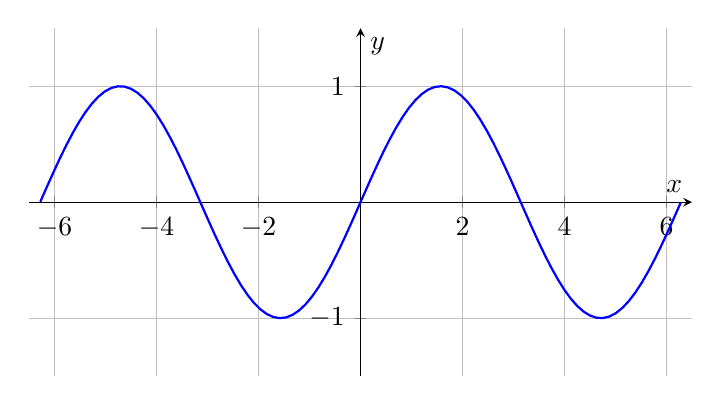
\begin{tikzpicture}
    \begin{axis}[
      width=10cm,
      height=6cm,
      axis lines=middle,
      xlabel=$x$,
      ylabel=$y$,
      xmin=-6.5, xmax=6.5,
      ymin=-1.5, ymax=1.5,
      grid=major,
      samples=100,
    ]
      \addplot[blue, thick, domain=-6.28:6.28] {sin(deg(x))};
    \end{axis}
  \end{tikzpicture}
  \end{center}
\end{frame}

\end{document}
